\documentclass{beamer}

\usetheme{Madrid}
\setbeamertemplate{navigation symbols}{}
\setbeamertemplate{caption}[numbered]


\usepackage{graphicx}
\usepackage{amsmath}
%\usepackage{xeCJK}
\usepackage{booktabs}
\usepackage{multirow}
\usepackage{tikz}
\usepackage{makecell}
\usepackage[notes,backend=bibtex,doi=false,isbn=false,url=false,eprint=false]{biblatex-chicago}
\bibliography{ref}
\usepackage{hyperref}
\usepackage{microtype}


\title[Democratic Peace Revisited]{The Theory of Democratic Peace Revisited \\ \large{Institutional Constraints or \textit{Pax Americana}}}
\author{Chen Zeng}
\institute[]{Department of Political Science \\ Renmin University of China}

\AtBeginSection[]
{
	\begin{frame}
		\frametitle{Section Overview}
		\tableofcontents[currentsection]
	\end{frame}
}

\begin{document}
	\maketitle
	
	\begin{frame}{Introduction}
		\begin{itemize}
			\item Why do states engage in warfare?
			\item If such question is too difficult to answer, let's consider another one: under which circumstances do states refrain from war engagement, i.e. under which circumstances do states maintain peace?
			\item Democratic Peace theory is one of the longest-standing explanations for interstate peace, arguing that democratic states do not fight wars with each other, compared to other regime dyads, \textit{ceteris paribus}.
			\item In normative political theories, democratic peace finds its origins in the writings of Mozi, Immanuel Kant, et al.
			\item In empirical studies, democratic peace is probably one of the most researched areas of comparative politics and international relations, for its practical importance in foreign policy making, methodological simplicity and consensus.
		\end{itemize}
	\end{frame}
	
	\begin{frame}{Contents}
		\tableofcontents
	\end{frame}

	\section{Conceptualizing Democratic Peace}
	
	\subsection{Militarized Disputes, War, and Peace}
	
	\begin{frame}{Militarized Disputes, War, and Peace}
		\begin{itemize}
			\item We define peace as the lack of interstate violence.
			\item Interstate violence takes on many forms. Wars might be the most common one, but full-on wars are scarce, and may lead us to reach biased conclusion.
			\item We instead operationalize peace as the lack of militarized interstate disputes, measured in the Correlates of War project.
		\end{itemize}
	\end{frame}

	\begin{frame}{Militarized Disputes, War, and Peace}
		\begin{figure}
			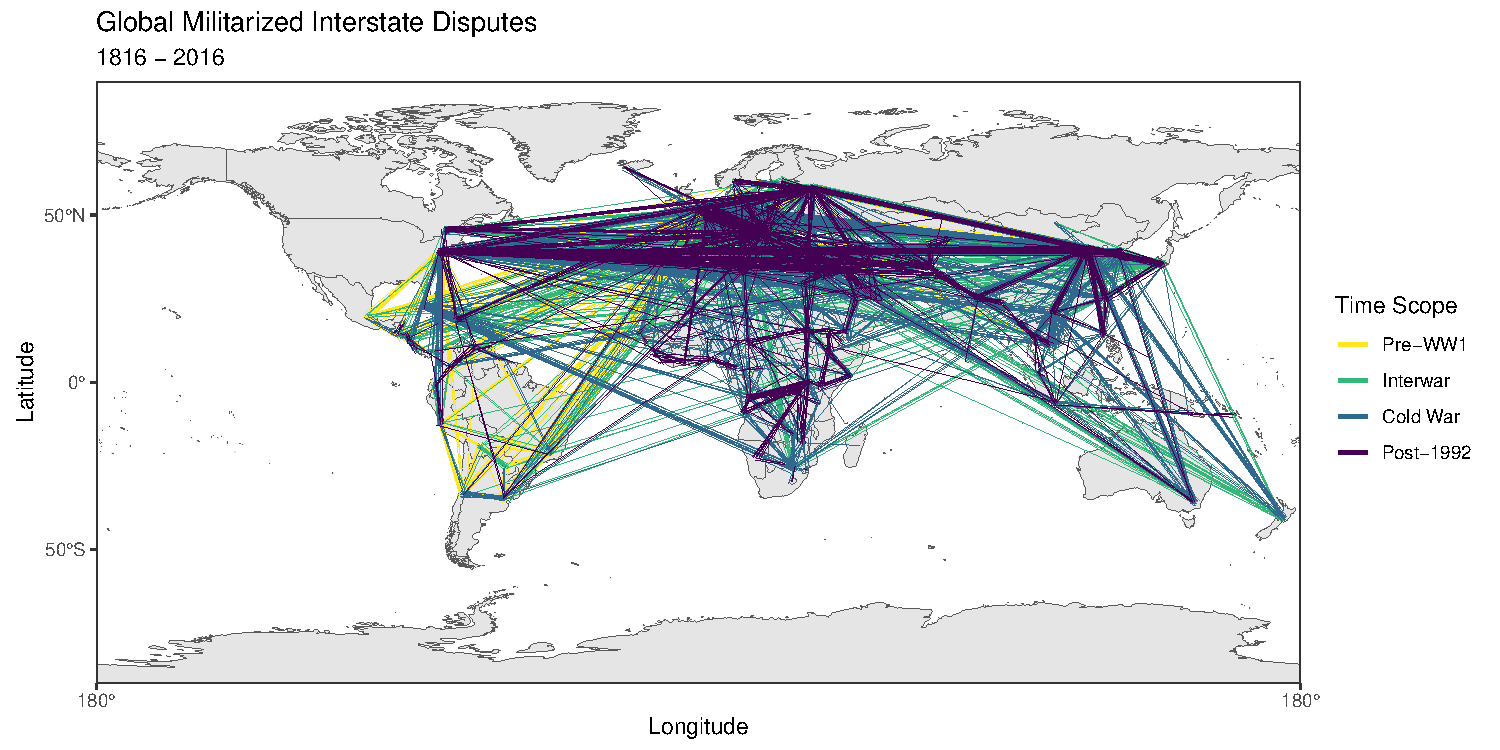
\includegraphics[width=\linewidth]{data/output/plots/all.pdf}
			\caption{Global MIDs Disaggregated by Time Periods (1816 -- 2016)}
		\end{figure}
	\end{frame}
	
	\subsection{Democracy: Normative and Empirical}
	
	\begin{frame}{Democracy: Normative and Empirical}
		\begin{itemize}
			\item If democracy does generate peace, what kind of democracy are we looking into?
			\item Etymologically, democracy stems from the ancient Greek word \textit{dēmokratía} (lit. rule of the people). Does the original meaning suffice to define how democracies should operate today? \footnote{See \cite{sartoriTheoryDemocracyRevisited1987}}
			\item While debates of normative definitions and values of democracy continue, our research demands an operational and measurable definition of democracy.
			\begin{itemize}
				\item \textit{Polity V}
				\item Freedom House (Political Rights, Civil Liberties)
				\item V-Dem
			\end{itemize}
		\end{itemize}
	\end{frame}

	\begin{frame}{Measuring Democracy with Polity Score}
		\begin{figure}
			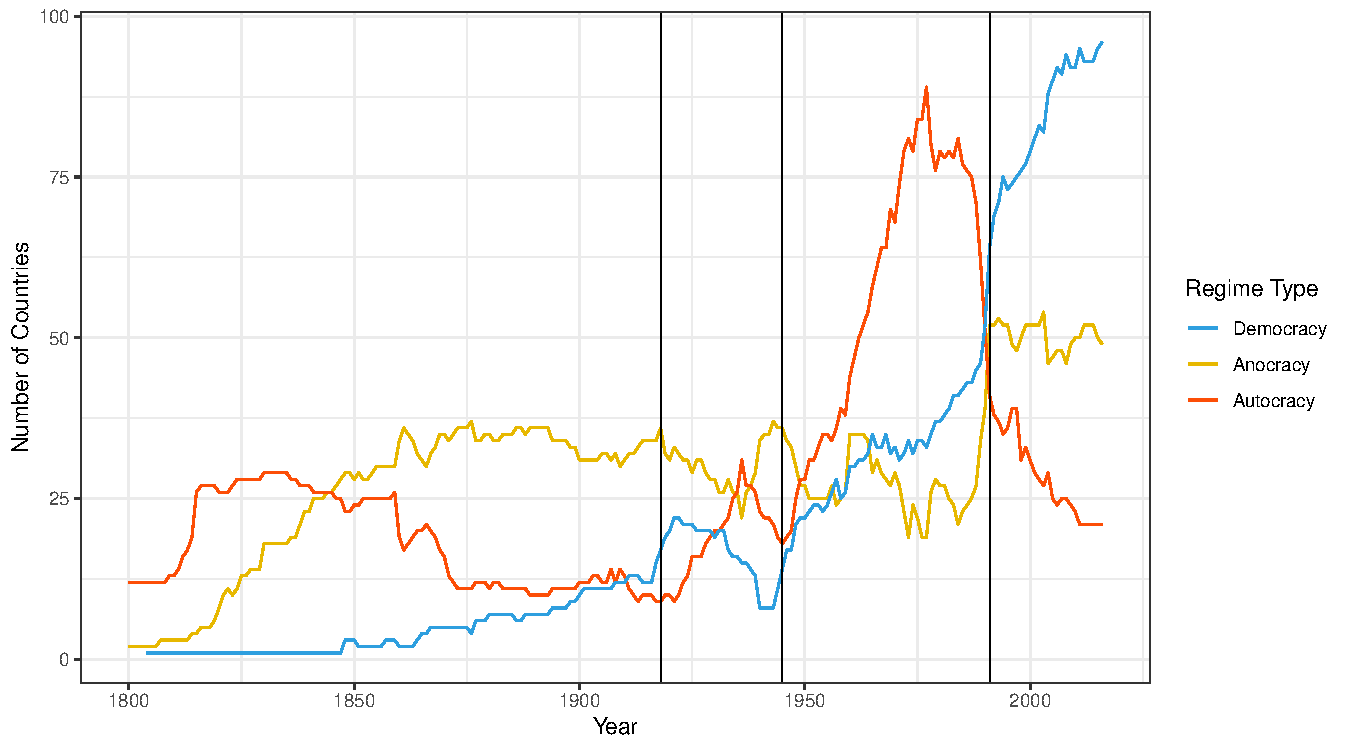
\includegraphics[width=\linewidth]{data/output/plots/polity_cnt.pdf}
			\caption{Number of Countries by Regime Type}
		\end{figure}
	\end{frame}

	\begin{frame}{Measuring Democracy with Polity Score}
		\begin{figure}
			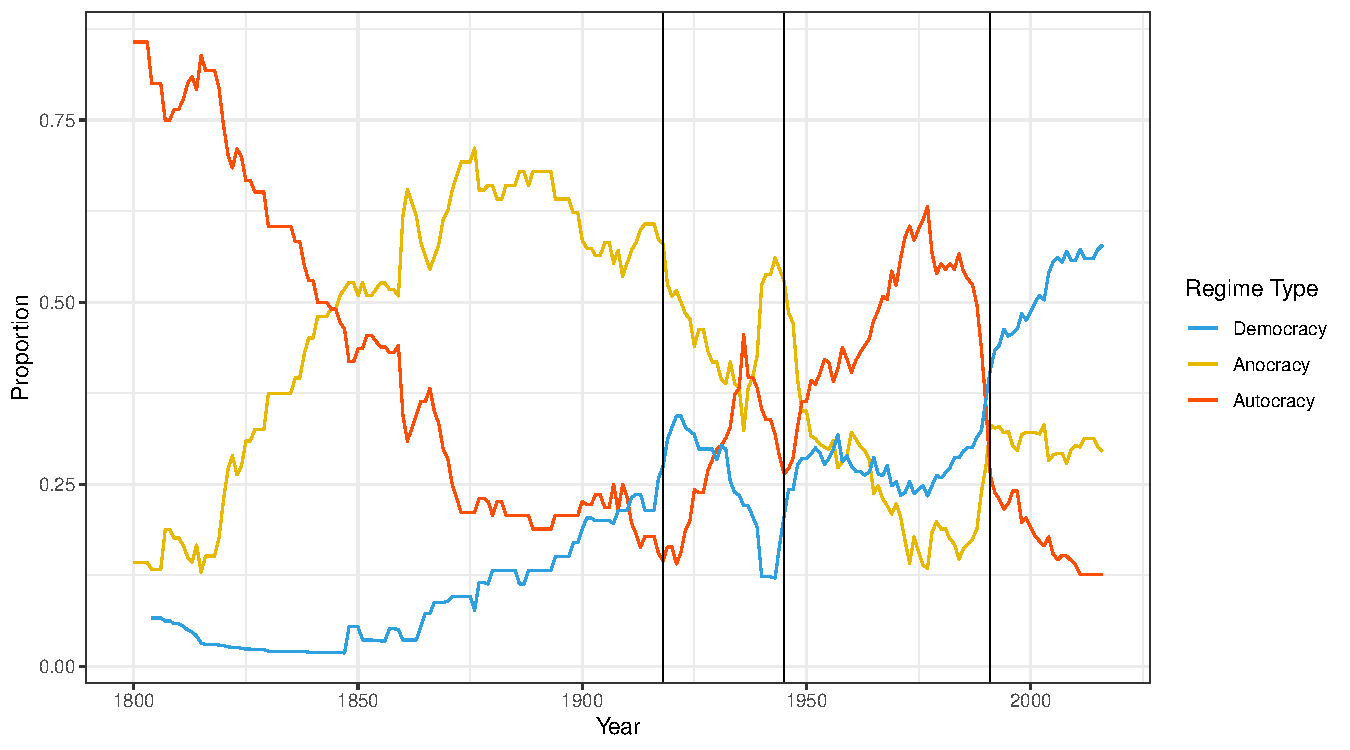
\includegraphics[width=\linewidth]{data/output/plots/polity_prp.pdf}
			\caption{Proportion of Regime Types in International Politics}
			\label{polity_proportion}
		\end{figure}
	\end{frame}
	
	\subsection{Operationalizing Democratic Peace}
	
	\begin{frame}{Operationalizing Democratic Peace}
		\begin{equation}
			logit(War) = \beta X
		\end{equation}
		\begin{description}
			\item[Outcome Variable] The probability of war breaking out in a dyad year; it is dichotomous, and takes on the value 0 or 1.
			\item[Explanatory Variable] A vector of predictors which we will discuss in the literature review section.
			\begin{itemize}
				\item Democracy scores,
				\item Great power hierarchy,
				\item Distance,
				\item Capacity difference...
			\end{itemize}
		\end{description}
	\end{frame}

	\section{Forty Years of Empirical Democratic Peace Study}
	
	\begin{frame}{Literature Review}
		\begin{itemize}
			\item As discussed by McDonald, \autocite{mcdonaldGreatPowersHierarchy2015} empirical research of democratic can be divided into four stages in the area of CP and IR.
			\begin{itemize}
				\item The first wave of empirical democratic peace study almost simultaneously revived with normative political philosophy in the 1970s and 1980s. Simple observations, descriptive and bivariate analysis were available in this period.
				\item More sophisticated methods were being employed in the second stage; research design was consolidated.
				\item Then followed by the unpacking black box of the mechanism of democratic peace.
				\item Alternative theories emerged to question the genesis and mechanism of democratic peace.
			\end{itemize}
		\end{itemize}
	\end{frame}
	
	\subsection{Revival of the Democratic Peace Thesis}
	
	\begin{frame}{Revival of the Democratic Peace Thesis}
		\begin{itemize}
			\item The first wave of empirical democratic peace study started to reexamine the intellectual legacy of political theorists. \autocite{doyleLiberalismWorldPolitics1986}
			\item Researchers observe that democratic states avoid fight war with each other. \autocite{chanMirrorMirrorWall1984}
			\item Such phenomenon can only be observed in state dyads, not single states. \autocite{maozRegimeTypesInternational1989}
			\item In most cases, only descriptive and bivariate analytic methods were being used. Regression analysis was rare. \autocite{rummelLibertarianismInternationalViolence1983}
			\item Problems?
		\end{itemize}
	\end{frame}
	
	\subsection{Consolidated Consensus of Methods and Research Design}
	
	\begin{frame}{Consolidated Consensus of Methods and Research Design}
		\begin{itemize}
			\item The second stage starts with consolidating research design decisions. Controlling variables were clearly defined, and preliminary causal mechanisms were properly modeled and discussed. \autocite{maozNormativeStructuralCauses1993}
			\begin{itemize}
				\item Normative causes: norms of compromise and cooperation prevent conflicts.
				\item Structural causes: complex political mobilization processes impose institutional constraints on leaders of two democracies confronting each other.
			\end{itemize}
			\item Furthermore, democracies can avoid escalation. \autocite{dixonDemocracyPeacefulSettlement1994}
			\item The unit of analysis has been agreed to be a state dyad, though evidence of monadic was observed in crisis emergence. \autocite{rousseauAssessingDyadicNature1996}
		\end{itemize}
	\end{frame}

	\begin{frame}{Consolidated Consensus of Methods and Research Design}
		\begin{itemize}
			\item Economic interdependence was sometimes considered, \autocite{onealClassicalLiberalsWere1997,russettTriangulatingPeaceDemocracy2001} but it was rendered spurious for failure to consider temporal dependence. \autocite{beckTakingTimeSeriously1998}
		\end{itemize}
	\end{frame}
	
	\subsection{Causal Mechanism of Democratic Peace}
	
	\begin{frame}{Causal Mechanism of Democratic Peace}
		\begin{itemize}
			\item This stage aimed to unpack the black box of democratic peace.
			\item Leaders in democratic countries avoid threatening use violence because of the domestic audience, \autocite{fearonDomesticPoliticalAudiences1994} while they can't avoid revealing this tendency to other non-democratic countries. \autocite{schultzDemocracyCoerciveDiplomacy2001}
			\item Democratic institutions also limit their leaders to allocate resources to fight costly long-term wars. \autocite{buenodemesquitaLogicPoliticalSurvival2003}
			\item The probability of democratic leaders losing office is relatively less dependent on the war outcome, as opposed to their counterparts in undemocratic countries. They are less likely to engage in wars. \autocite{debsRegimeTypeFate2010}
		\end{itemize}
	\end{frame}

	\begin{frame}{Causal Mechanism of Democratic Peace}
		\begin{itemize}
			\item From a social constructivist perspective, democratic states adopt non-violent and compromise-oriented behaviors with other democracies, while interacting with non-democracies with enmity under the realist assumption of international anarchy. \autocite{risse-kappenDemocraticPeaceWarlike1995}
			\item The peace between or among democracies depends on norms of nonviolent dispute resolution, politically educated public, and free press that keep the people informed. \autocite{hayesSecuritizationSocialIdentity2012}
		\end{itemize}
	\end{frame}
	
	\subsection{Emergence of Alternative Theoretical Explanations}
	
	\begin{frame}{Emergence of Alternative Theoretical Explanations}
		\begin{itemize}
			\item Democratic peace theory has also been heavily challenged.
			\item For example, unsuccessful democratic transition can cause militarized conflicts, and democratic peace seems to only restricted to consolidated democracies. \autocite{mansfieldElectingFightWhy2005}
			\item Reverse causation?
		\end{itemize}
	\end{frame}

	\begin{frame}{Emergence of Alternative Theoretical Explanations}
		\begin{figure}
			\centering
			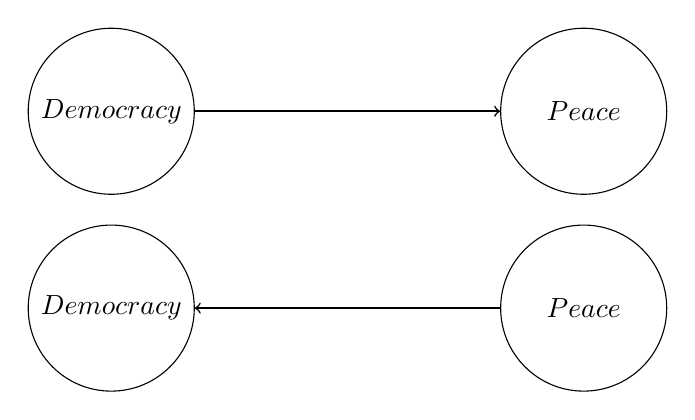
\begin{tikzpicture}[node distance = 3cm, auto]
				\node[circle,
				minimum width = 60pt,
				minimum height = 60pt, draw=black] (1) at(0,0){$Democracy$};
				\node[circle,
				minimum width = 60pt,
				minimum height = 60pt, draw=black] (2) at(6,0){$Peace$};
				\node[circle,
				minimum width = 60pt,
				minimum height = 60pt, draw=black] (3) at(0,-2.5){$Democracy$};
				\node[circle,
				minimum width = 60pt,
				minimum height = 60pt, draw=black] (4) at(6,-2.5){$Peace$};
				\draw[line width=0.2mm,->] (1) -- (2);
				\draw[line width=0.2mm,->] (4) -- (3);
			\end{tikzpicture}
			\caption{Reverse Causation of Democratic Peace Theory}
		\end{figure}
	\end{frame}

	\begin{frame}
		\begin{itemize}
			\item The cost of treating regime types as exogenous?---Refer to Figure \ref{polity_proportion}.
			\item Great powers' hegemony in international politics, \autocite{nariznyAngloAmericanPrimacyGlobal2012} power shifts, \autocite{gunitskyShocksWavesHegemonic2014} and the shaping of regime types as a result of great power alliance \autocite{brinksDiffusionNoIllusion2006,boixDemocracyDevelopmentInternational2011} challenge the exogeneity of democracy in most countries around the world.
		\end{itemize}
	\end{frame}

	\section{Analysis}
	
	\subsection{Tracing the Mechanism of Democratic Peace}
	
	\begin{frame}{Tracing the Mechanism of Democratic Peace}
		\centering\Large Example of the Bangladesh War
	\end{frame}
	
	\subsection{Disaggregating the Democratic Peace}
	
	\begin{frame}{Disaggregating the Democratic Peace}
		\centering\large As seen in the literature review, is the correlation between democracy and peace weak prior to WWI?
	\end{frame}
	
	\begin{frame}{Disaggregating the Democratic Peace}
	\begin{figure}
		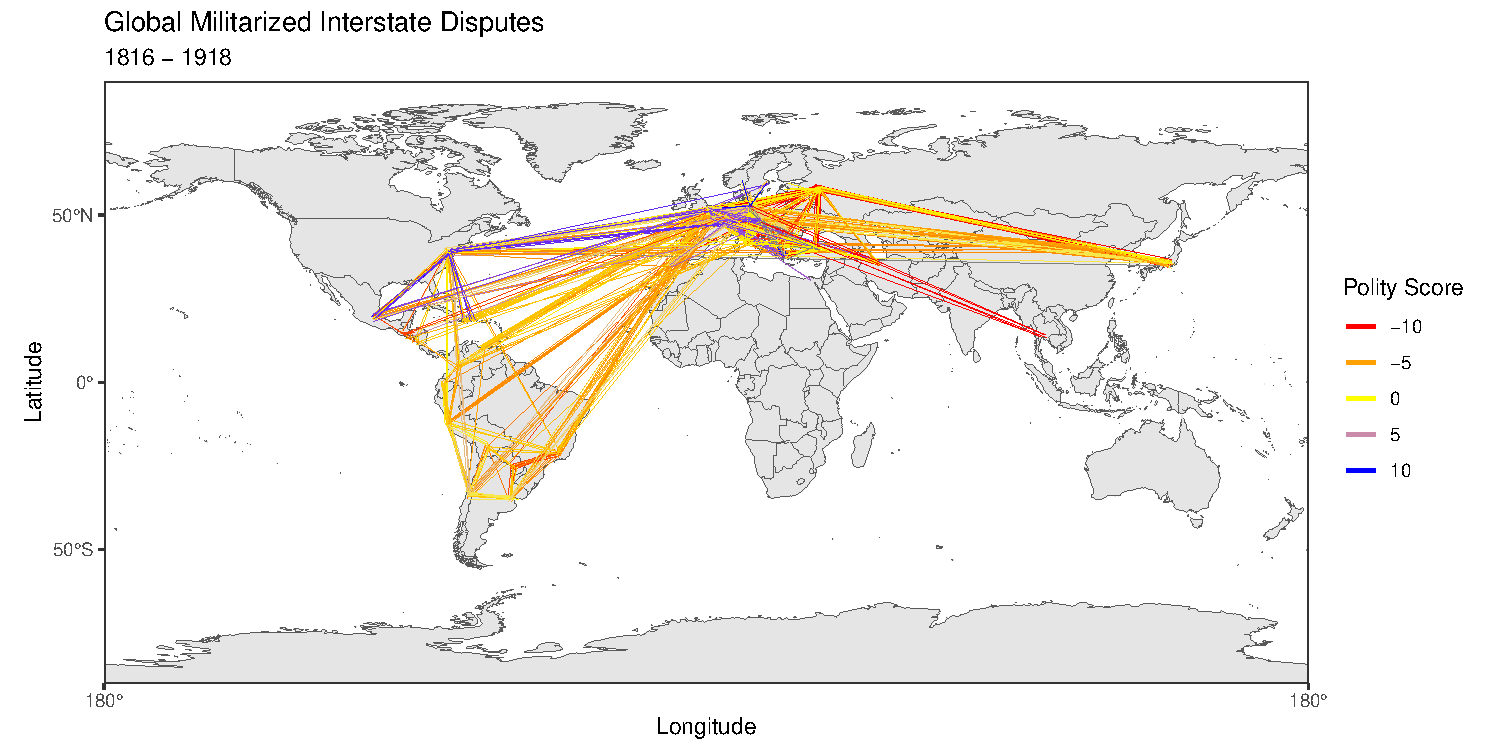
\includegraphics[width=\linewidth]{data/output/plots/preww1.pdf}
		\caption{Global Militarized Interstate Disputes (1816 -- 1918)}
	\end{figure}
	\end{frame}

	\begin{frame}{Disaggregating the Democratic Peace}
	\begin{figure}
		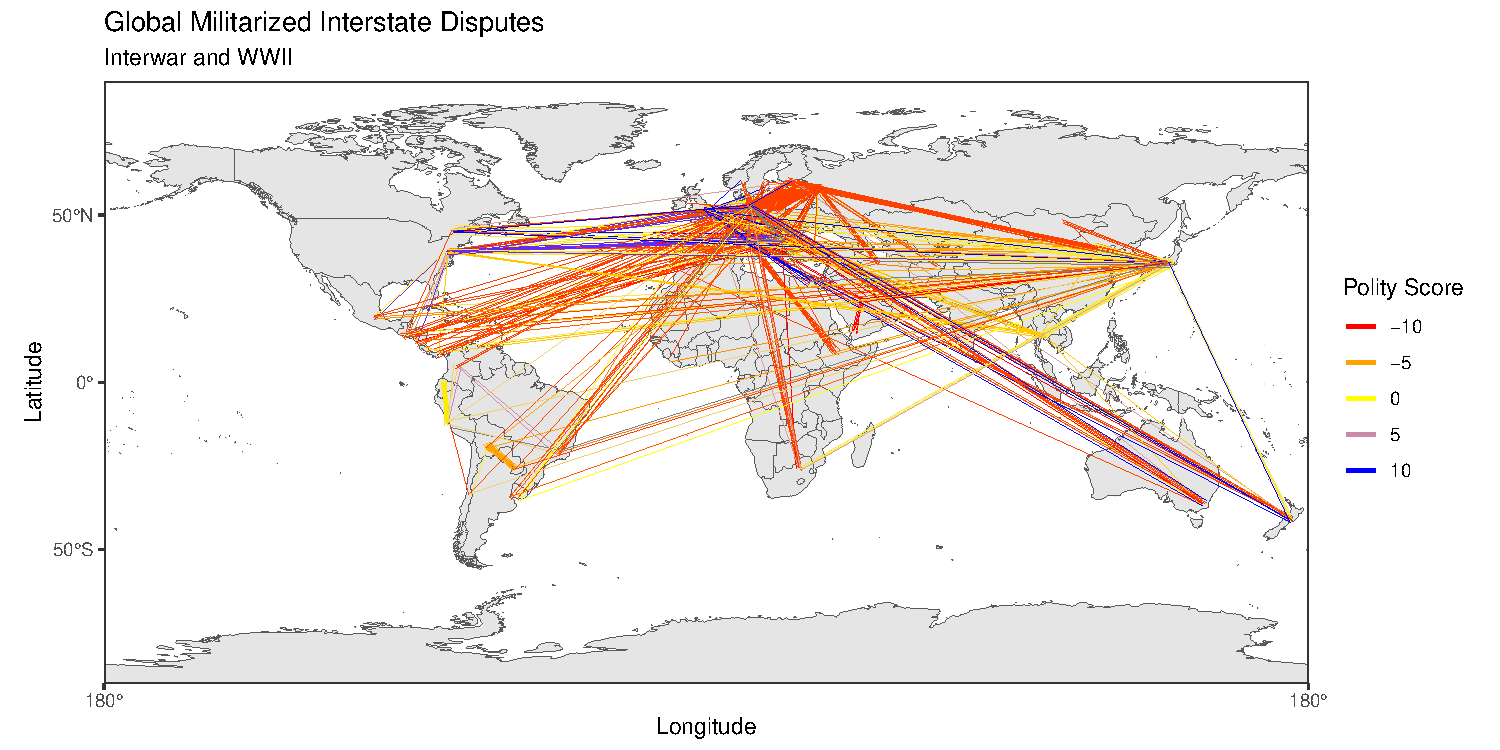
\includegraphics[width=\linewidth]{data/output/plots/interwar.pdf}
		\caption{Global Militarized Interstate Disputes (1919 -- 1945)}
	\end{figure}
	\end{frame}

	\begin{frame}{Disaggregating the Democratic Peace}
	\begin{figure}
		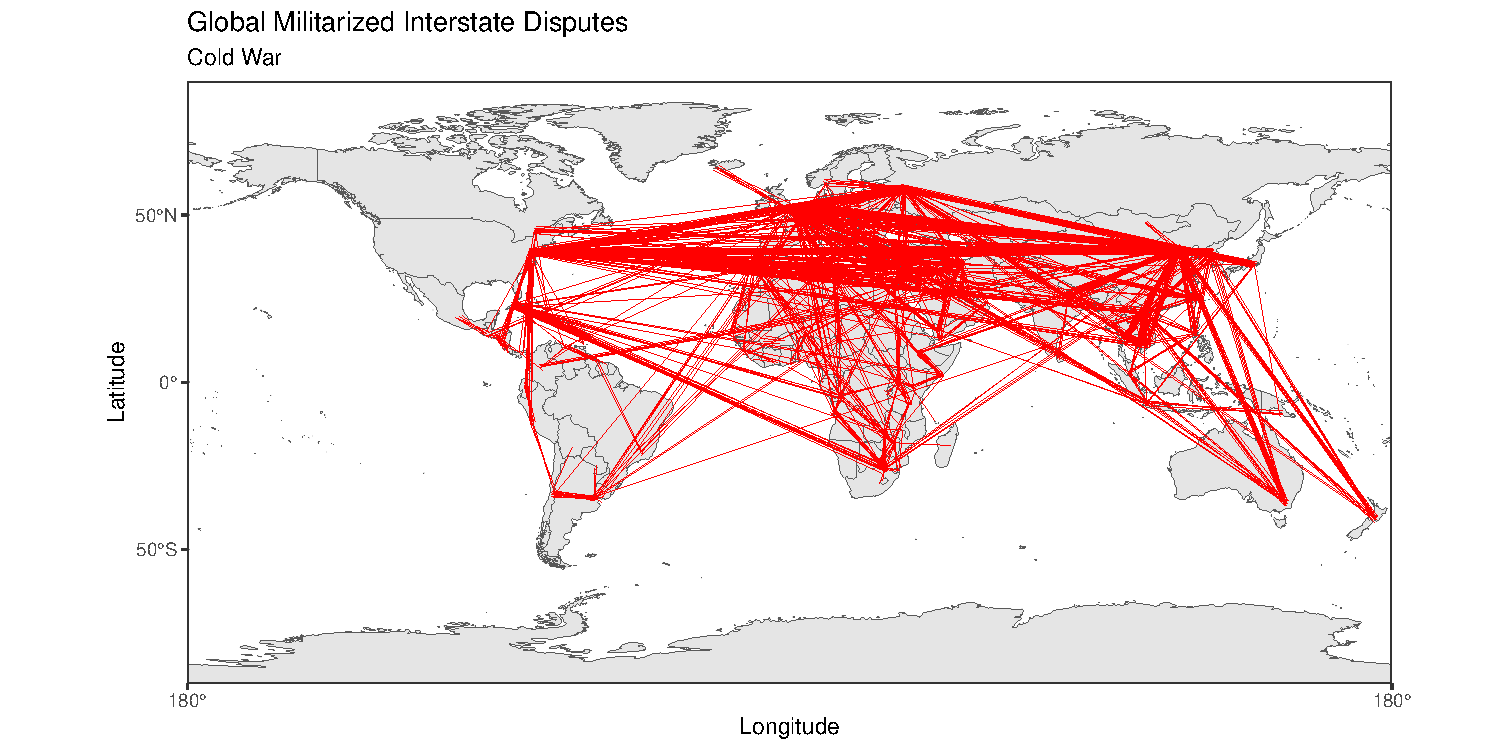
\includegraphics[width=\linewidth]{data/output/plots/coldwar.pdf}
		\caption{Global Militarized Interstate Disputes (1946 -- 1991)}
	\end{figure}
	\end{frame}


	\begin{frame}{Disaggregating the Democratic Peace}
		\begin{figure}
			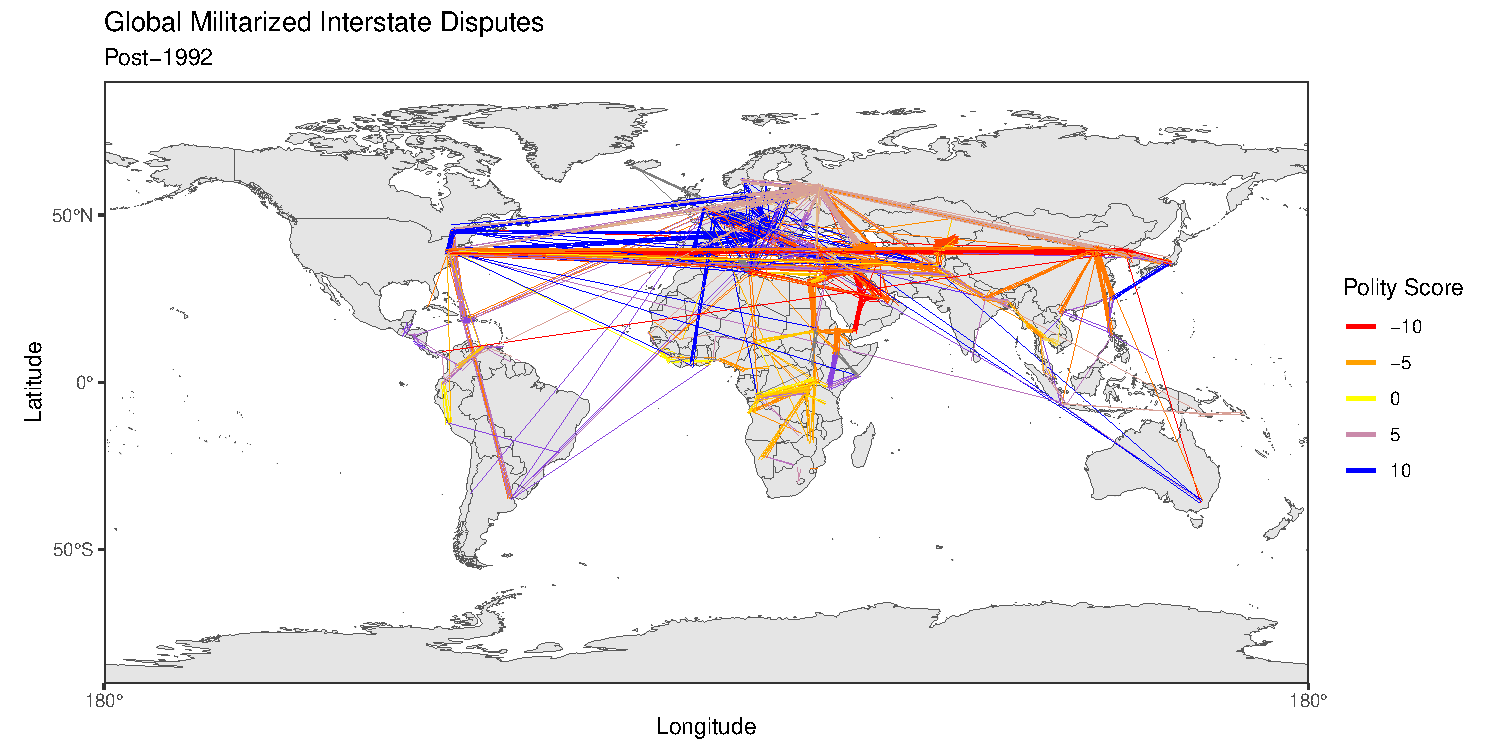
\includegraphics[width=\linewidth]{data/output/plots/post1992.pdf}
			\caption{Global Militarized Interstate Disputes (1992 -- 2016)}
		\end{figure}
	\end{frame}

	\begin{frame}{Disaggregating the Democratic Peace}
		\begin{itemize}
			\item Let's model the correlation between democracy and peace formally, disaggregated by the time scope(pre-WWI, interwar and WWII, Cold War, and post-1992).
			\item We have two explanatory variables: democracy (measured as the lower polity score in a dyad), and great power (if one of the state in the dyad is a great power defined in the COW project).
			\item We control dyadic alliance, intercapital distance, contiguity, and capacity ratio. It is common practice as discussed in literature review.
			\item Since the outcome variable is dichotomous, we can use logistic regression to model this problem.
			\item As a type of Generalized Linear Models (GLMs), logistic regression uses a link function to transform the range of the outcome variable to $[0,1]$.
		\end{itemize}
	\end{frame}

	\begin{frame}{Disaggregating the Democratic Peace}
		\begin{equation}
			logit(Y)=ln(\frac{Y}{1-Y})=\beta_0 + X\beta
		\end{equation}
		
		\begin{equation}
			\text{equivalent of }Y=\frac{e^{\beta_0 + X\beta}}{1+e^{\beta_0 + X\beta}},
			Y \sim [0,1]
		\end{equation}
	
		\begin{itemize}
			\item Mathematically, we have the following model:
		\end{itemize}
		
		\begin{equation}
			\begin{aligned}
				logit(MID) = & \beta_0  + \beta_1 \times Democracy + \beta_2 \times Great Power + \\
				             & \beta_3 \times Alliance + \beta_4 \times ln(Distance) + \\
				             & \beta_5 \times Contiguity + \beta_6 \times Cap. Ratio
			\end{aligned}
		\end{equation}
	
		\begin{itemize}
			\item We use MLE to estimate parameters in the model, as MCMC converges extremely slowly due to large sample size, and we don't have to incorporate priors here.
		\end{itemize}
	\end{frame}


	\begin{frame}{Disaggregating the Democratic Peace}
		
% Table created by stargazer v.5.2.3 by Marek Hlavac, Social Policy Institute. E-mail: marek.hlavac at gmail.com
% Date and time: 二, 3月 29, 2022 - 00时23分01秒
\begin{table}[!htbp] \centering 
  \caption{Disaggregated MIDs 1816 -- 2016\label{dis_mid}} 
  
\tiny 
\begin{tabular}{lccccc} 
\toprule
 & \multicolumn{5}{c}{Outcome Variable: MID} \\ 
\cmidrule{2-6} 

 & All Years & Pre-WW1 & Interwar and WW2 & Cold War & Post-1992 \\ 

\midrule
 Democracy & $-$0.077$^{***}$ & 0.040$^{***}$ & $-$0.076$^{***}$ & $-$0.122$^{***}$ & $-$0.077$^{***}$ \\ 
& (0.002) & (0.006) & (0.005) & (0.003) & (0.003) \\ 
Great Power & 0.963$^{***}$ & 1.501$^{***}$ & 1.942$^{***}$ & 1.042$^{***}$ & 1.363$^{***}$ \\ 
& (0.027) & (0.071) & (0.068) & (0.055) & (0.066) \\ 
Dyadic Alliance & $-$0.476$^{***}$ & $-$1.695$^{***}$ & $-$0.355$^{***}$ & $-$0.353$^{***}$ & $-$0.640$^{***}$ \\ 
& (0.029) & (0.098) & (0.081) & (0.043) & (0.059) \\ 
$ln(Intercapital Distance)$ & $-$0.131$^{***}$ & $-$0.023 & $-$0.129$^{***}$ & $-$0.123$^{***}$ & $-$0.197$^{***}$ \\ 
& (0.015) & (0.036) & (0.041) & (0.022) & (0.028) \\ 
Contiguity & 2.874$^{***}$ & 1.672$^{***}$ & 1.859$^{***}$ & 3.241$^{***}$ & 3.528$^{***}$ \\ 
& (0.039) & (0.093) & (0.098) & (0.057) & (0.080) \\ 
Capacity Ratio & $-$0.019$^{**}$ & $-$0.021 & 0.111$^{***}$ & $-$0.057$^{***}$ & $-$0.169$^{***}$ \\ 
& (0.008) & (0.022) & (0.020) & (0.013) & (0.017) \\ 
Intercept & $-$4.804$^{***}$ & $-$5.230$^{***}$ & $-$4.416$^{***}$ & $-$5.356$^{***}$ & $-$4.082$^{***}$ \\ 
& (0.225) & (0.550) & (0.632) & (0.333) & (0.431) \\ 
\midrule
Observations & 1,955,623 & 126,541 & 115,980 & 865,565 & 847,537 \\ 
Log Likelihood & $-$39,915.260 & $-$4,812.858 & $-$4,787.485 & $-$18,945.180 & $-$10,046.850 \\ 
Akaike Inf. Crit. & 79,844.520 & 9,639.715 & 9,588.971 & 37,904.370 & 20,107.690 \\ 
\bottomrule \\[-1.8ex] 
\textit{Note:}  & \multicolumn{5}{r}{$^{*}$p$<$0.1; $^{**}$p$<$0.05; $^{***}$p$<$0.01} \\ 
\end{tabular} 
\end{table} 

	\end{frame}
	
	\subsection{Democratic Peace and Great Power Hierarchy}
	
	\begin{frame}{Democratic Peace and Great Power Hierarchy}
		\begin{itemize}
			\item As seen in the previous table, democracy and MID are positively correlated. This means democratic peace didn't exist before WWI.
			\item Let's model great power supported democracies to examine if the so-called democratic peace is actually generated by great power hierarchies.
		\end{itemize}
	\end{frame}
	
	\begin{frame}{Democratic Peace and Great Power Hierarchy}
		
% Table created by stargazer v.5.2.3 by Marek Hlavac, Social Policy Institute. E-mail: marek.hlavac at gmail.com
% Date and time: 二, 3月 29, 2022 - 00时23分01秒
\begin{table}[!htbp] \centering 
	\caption{``Great Power Supported'' Democracies and Democratic Peace\footnotemark} 
	\label{gpdem} 
	\scriptsize
	\begin{tabular}{lcccc} 
		\toprule
		& \multicolumn{4}{c}{Outcome Variable} \\ 
		\cmidrule{2-5}
		& \multicolumn{2}{c}{1919 -- 1945} &
		  \multicolumn{2}{c}{1946 -- 1991} \\
		& MID & FATALMID & MID & FATALMID \\ 
		\midrule
		Democracy & $-0.026^{*}$ & & $-0.010$       & $-0.007$      \\
		          & $(0.015)$    & & $(0.017)$      & $(0.033)$     \\
		GPDEM     & $5.258^{**}$ & & $2.871^{***}$  & $7.311^{***}$ \\
		          & $(2.321)$    & & $(0.958)$      & $(1.561)$     \\
		GPDEM$\times$Democracy
		          & $-1.031^{**}$& & $-0.384^{***}$ & $-1.035^{***}$\\
		          & $(0.357)$    & & $(0.112)$      & $(0.156)$     \\
		\midrule
		Observations
		          & $46,000$     & & $311,489$      & $311,189$     \\
		 
		\bottomrule \\[-1.8ex] 
		\textit{Note:}  & \multicolumn{4}{r}{$^{*}$p$<$0.1; $^{**}$p$<$0.05; $^{***}$p$<$0.01}
	\end{tabular} 
\footnotetext{\cite{mcdonaldGreatPowersHierarchy2015}}
\end{table} 

	\end{frame}
		
	\begin{frame}{Great Power Hierarchy as A Confounder}
		\begin{figure}
			\centering
			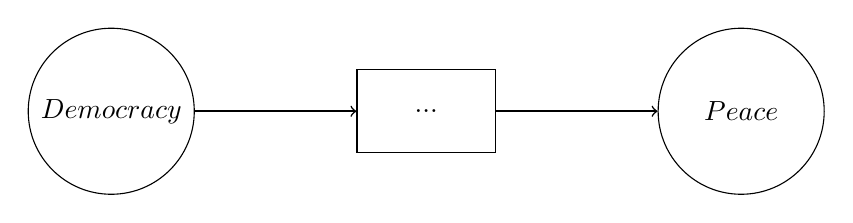
\begin{tikzpicture}[node distance = 3cm, auto]
				\node[circle,
				minimum width = 60pt,
				minimum height = 60pt, draw=black] (1) at(0,0){$Democracy$};
				\node[circle,
				minimum width = 60pt,
				minimum height = 60pt, draw=black] (2) at(8,0){$Peace$};
				\node (rect) [
				minimum width = 50pt,
				minimum height = 30pt, draw=black] (3) at(4,0){$...$};
				\draw[line width=0.2mm,->] (1) -- (3);
				\draw[line width=0.2mm,->] (3) -- (2);
			\end{tikzpicture}
			\caption{Causal Diagram of Common Research Design}
		\end{figure}
	\end{frame}

	\begin{frame}{Great Power Hierarchy as A Confounder}
		\begin{figure}
			\centering
			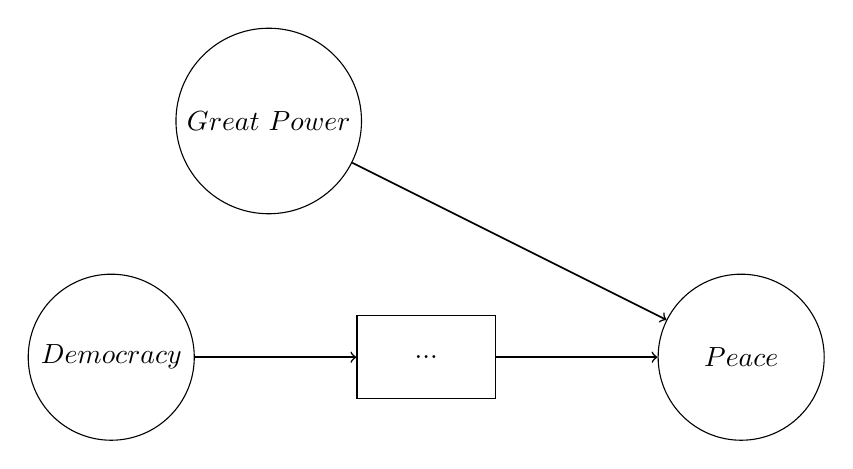
\begin{tikzpicture}[node distance = 3cm, auto]
				\node[circle,
				minimum width = 60pt,
				minimum height = 60pt, draw=black] (1) at(0,0){$Democracy$};
				\node[circle,
				minimum width = 60pt,
				minimum height = 60pt, draw=black] (2) at(8,0){$Peace$};
				\node (rect) [
				minimum width = 50pt,
				minimum height = 30pt, draw=black] (3) at(4,0){$...$};
				\node[circle,
				minimum width = 60pt,
				minimum height = 60pt, draw=black] (4) at(2,3){$Great\ Power$};
				\draw[line width=0.2mm,->] (1) -- (3);
				\draw[line width=0.2mm,->] (3) -- (2);
				\draw[line width=0.2mm,->] (4) -- (2);
			\end{tikzpicture}
			\caption{Causal Diagram Modeling Great Powers}
		\end{figure}
	\end{frame}

	\begin{frame}{Great Power Hierarchy as A Confounder}
		\begin{figure}
			\centering
			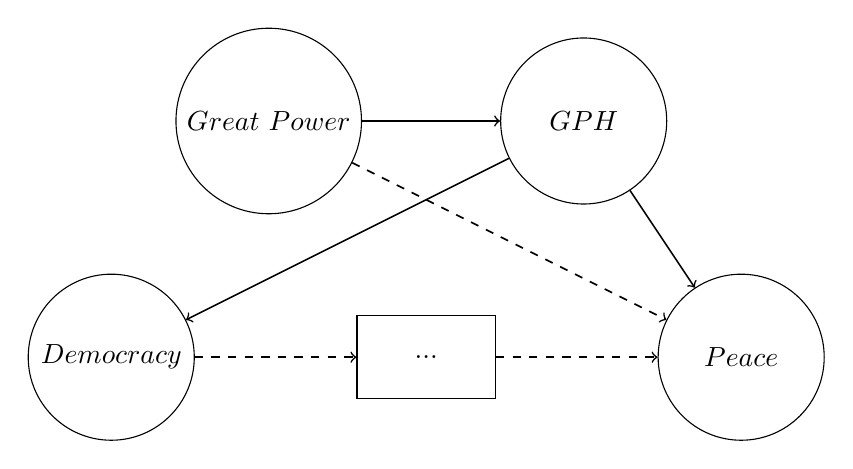
\begin{tikzpicture}[node distance = 3cm, auto]
				\node[circle,
				minimum width = 60pt,
				minimum height = 60pt, draw=black] (1) at(0,0){$Democracy$};
				\node[circle,
				minimum width = 60pt,
				minimum height = 60pt, draw=black] (2) at(8,0){$Peace$};
				\node (rect) [
				minimum width = 50pt,
				minimum height = 30pt, draw=black] (3) at(4,0){$...$};
				\node[circle,
				minimum width = 60pt,
				minimum height = 60pt, draw=black] (4) at(2,3){$Great\ Power$};
				\node[circle,
				minimum width = 60pt,
				minimum height = 60pt, draw=black] (5) at(6,3){$GPH$};
				\draw[dashed,line width=0.2mm,->] (1) -- (3);
				\draw[dashed,line width=0.2mm,->] (3) -- (2);
				\draw[dashed,line width=0.2mm,->] (4) -- (2);
				\draw[line width=0.2mm,->] (4) -- (5);
				\draw[line width=0.2mm,->] (5) -- (1);
				\draw[line width=0.2mm,->] (5) -- (2);
			\end{tikzpicture}
			\caption{Causal Diagram Modeling Great Power Hierarchy}
		\end{figure}
	\end{frame}
	
	\section{Conclusion}
	
	\begin{frame}{Conclusion}
		\begin{itemize}
			\item The phenomenon called democratic peace did \textit{not} exist prior to WWI.
			\item The endogeneity of regime types confounds the statistical relationship between democracy and peace. When it is modeled, the correlation collapses. This means that democratization in the immediate aftermath of two world wars and the Cold War was managed by the great powers; they generate similar regime types and peace in their hierarchies.
			\item The democratic peace we know today is, in fact, \textit{Pax Americana}.
			\item International politics is still constructed and operated by great powers. \autocite{mcdonaldGreatPowersHierarchy2015}
		\end{itemize}
	\end{frame}
	
	\begin{frame}
		\begin{block}{What now?}
			{\large To realize the relative validity of one's convictions and yet stand for them unflinchingly is what distinguishes a civilized man from a barbarian.}
			\vskip5mm
			\hspace*\fill{\small--- Joseph Schumpeter, \textit{Capitalism, Socialism, and Democracy}}
		\end{block}
		\centering\LARGE Thanks!
	\end{frame}

	\begin{frame}[allowframebreaks]{Bibliography}
		\nocite{*}
		\printbibliography
	\end{frame}
	
\end{document}